\documentclass[twocolumn,a4j]{jsarticle}
\setlength{\topmargin}{-20.4cm}
\setlength{\oddsidemargin}{-10.4mm}
\setlength{\evensidemargin}{-10.4mm}
\setlength{\textwidth}{18cm}
\setlength{\textheight}{26cm}

\usepackage[top=15truemm,bottom=25truemm,left=20truemm,right=20truemm]{geometry}
\usepackage[latin1]{inputenc}
\usepackage{amsmath}
\usepackage{amsfonts}
\usepackage{amssymb}
\usepackage[dvipdfmx]{graphicx}
\usepackage[dvipdfmx]{color}
\usepackage{listings}
\usepackage{listings,jvlisting}
\usepackage{geometry}
\usepackage{framed}
\usepackage{color}
\usepackage[dvipdfmx]{hyperref}
\usepackage{ascmac}
\usepackage{enumerate}
\usepackage{tabularx}
\usepackage{cancel}
\usepackage{scalefnt}

\renewcommand{\figurename}{fig.}
\renewcommand{\tablename}{table }

\lstset{
basicstyle={\ttfamily},
identifierstyle={\small},
commentstyle={\smallitshape},
keywordstyle={\small\bfseries},
ndkeywordstyle={\small},
stringstyle={\small\ttfamily},
frame={tb},
breaklines=true,
columns=[l]{fullflexible},
xrightmargin=0zw,
xleftmargin=3zw,
numberstyle={\scriptsize},
stepnumber=1,
numbersep=1zw,
lineskip=-0.5ex
}

\makeatletter
\def\@maketitle
{
\begin{center}
{\LARGE \@title \par}
\end{center}
\begin{flushright}
{\large \@date}\\
{\large{京都工芸繊維大学 工芸科学科 機械工学課程}}\\
{\large \@author}
\end{flushright}
\par\vskip 1.5em
}
\makeatother

\setcounter{tocdepth}{3}

\author{来代 勝胤}
\title{令和3年度 9月度 報告書}
\date{2021/9/8}

\begin{document}
\columnseprule=0.1mm

\maketitle
\section*{報告内容}
\begin{enumerate}[1.]
    \item ノイズの除去方法
    \item 水流の起動・停止時刻の特定
    \item ドリフトの補正
    \item 補正結果と傾向
\end{enumerate}
\section{ノイズの除去方法について}
データの事前処理として,移動平均法,中央値法を利用した.
今回は任意の点において前後5点の合計11点を用いた移動平均をとり,
そのデータを解析対象した.
\par
なお,当資料におけるグラフには2021年8月6日(金)に実施した"Normal"モデルの実験データを用いている.
\begin{figure}[htbp]
    \footnotesize
    \begin{center}
        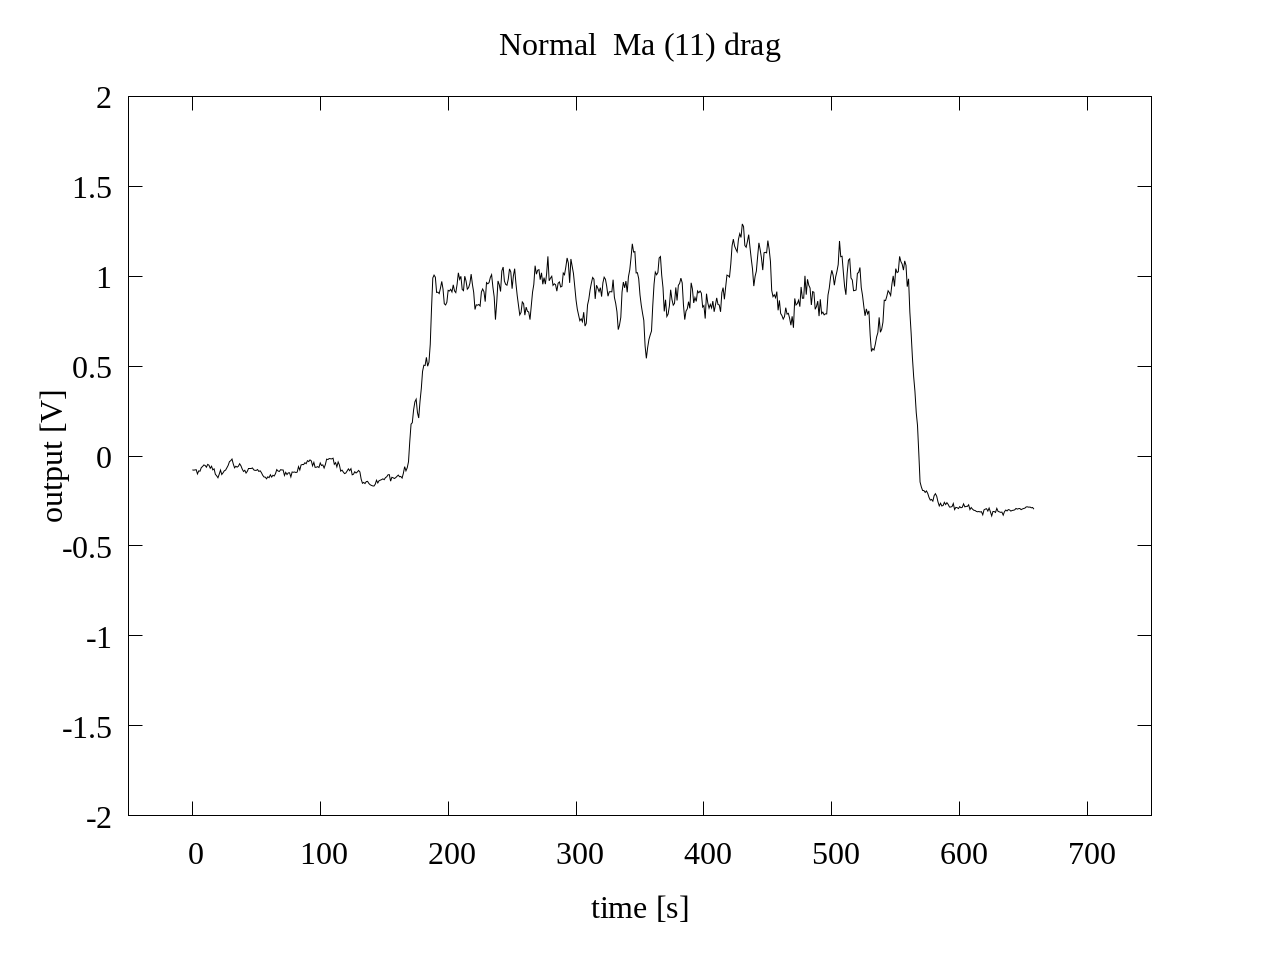
\includegraphics[width=80mm]{images/Normal_ma(11)_drag_01.png}
        \caption{Moving average method}
        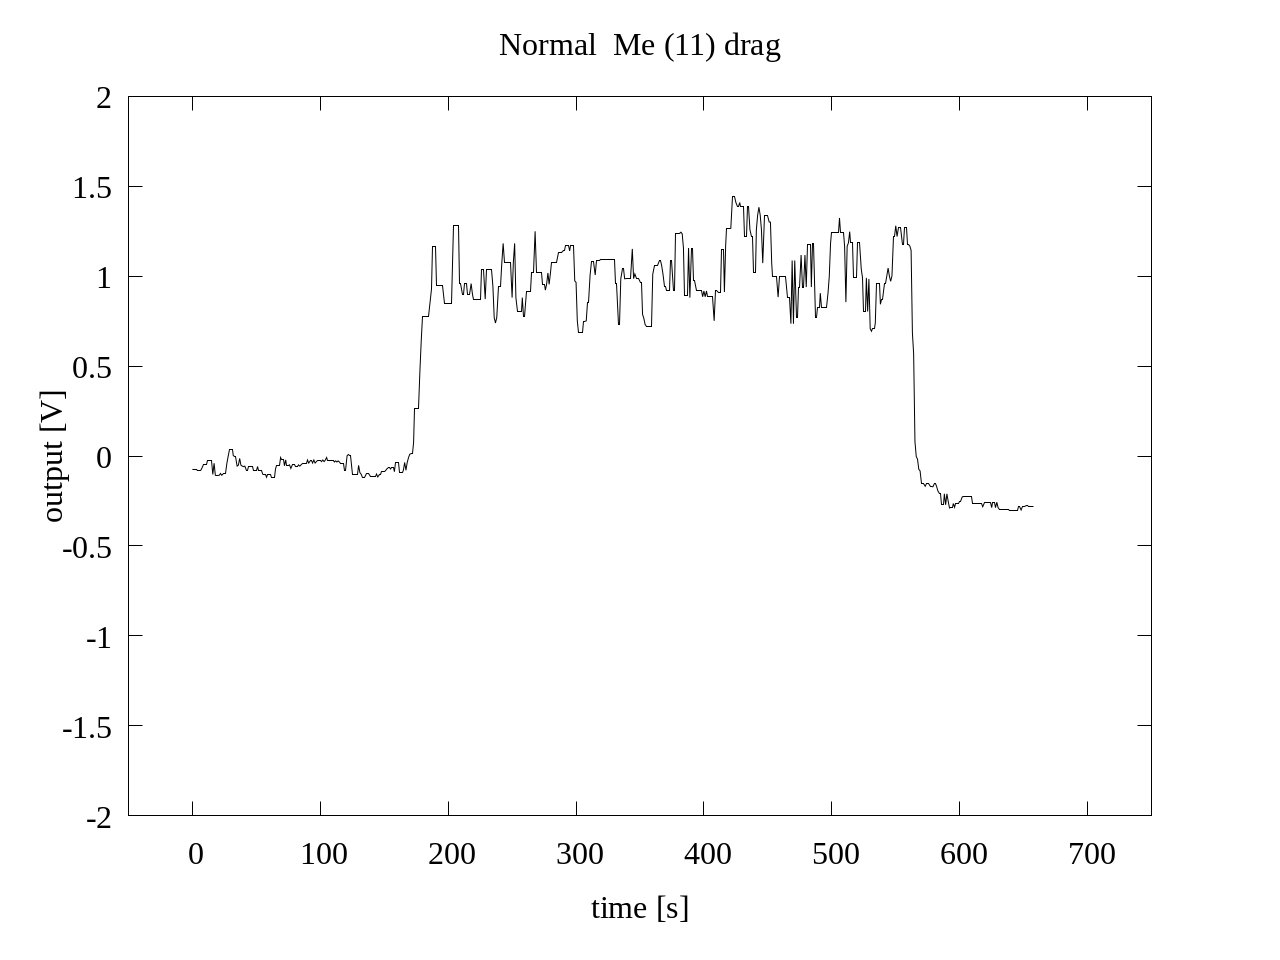
\includegraphics[width=80mm]{images/Normal_me(11)_drag_01.png}
        \caption{Median method}
    \end{center}
\end{figure}
\section{水流の起動・停止時刻の特定}
データの解析を行う前に,
回流水槽の水流の起動及び停止時刻を特定する必要がある.
特定に際して,後の処理を考慮した時刻を採用している.

\subsection{起動・停止時刻特定の条件}
\begin{itemize}
    \item [$\blacksquare$] \textgt{起動時刻の特定}
        \begin{itemize}
            \item [$\bullet$] 大きく上昇する直前の時刻を捉えたい
            \item [$\bullet$] Dragデータで特定し,Liftデータにも利用
        \end{itemize}
    \item [$\blacksquare$] \textgt{停止時刻の特定}
        \begin{itemize}
            \item [$\bullet$] 降下後の時刻を捉えたい
            \item [$\bullet$] Dragデータで特定し,Liftデータにも利用
        \end{itemize}
\end{itemize}
\subsection{起動時刻特定のアルゴリズム}
\begin{enumerate}[(1)]
    \item 任意の時刻 t(s) について,前部(n=90)と後部(n=10)を指定する.
    \item 前部の最大値の特定及び後部の平均値を算出する.
    \item 後部の最大値が前部の平均値を上回った場合の時刻 t(s) を"起動時刻"として採用する.
\end{enumerate}
\begin{figure}[htbp]
    \footnotesize
    \begin{center}
        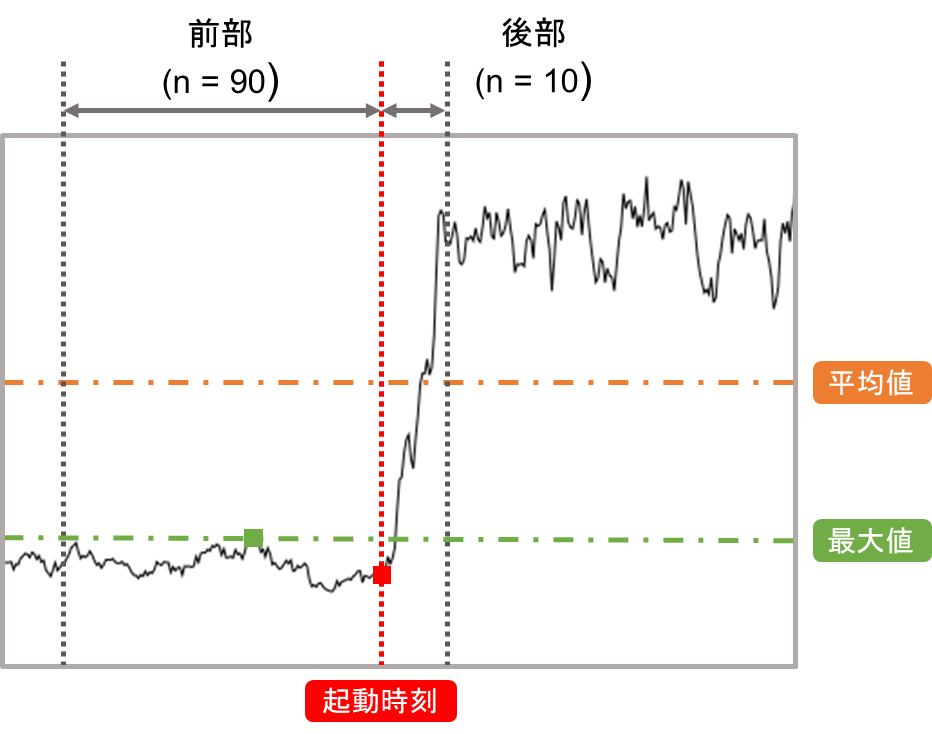
\includegraphics[width=80mm]{images/start.png}
        \caption{Method fo detecting start time}
    \end{center}
\end{figure}
\subsection{停止時刻特定のアルゴリズム}
\begin{enumerate}[(1)]
    \item 任意の時刻 t(s) について,前部(n=120)と後部(n=10)を指定する.
    \item 前部の最小値及び後部の平均値を特定する.
    \item 後部の平均値が前部の最小値を下回った場合の時刻 t(s) を"停止時刻"として採用する.
\end{enumerate}
\begin{figure}[htbp]
    \footnotesize
    \begin{center}
        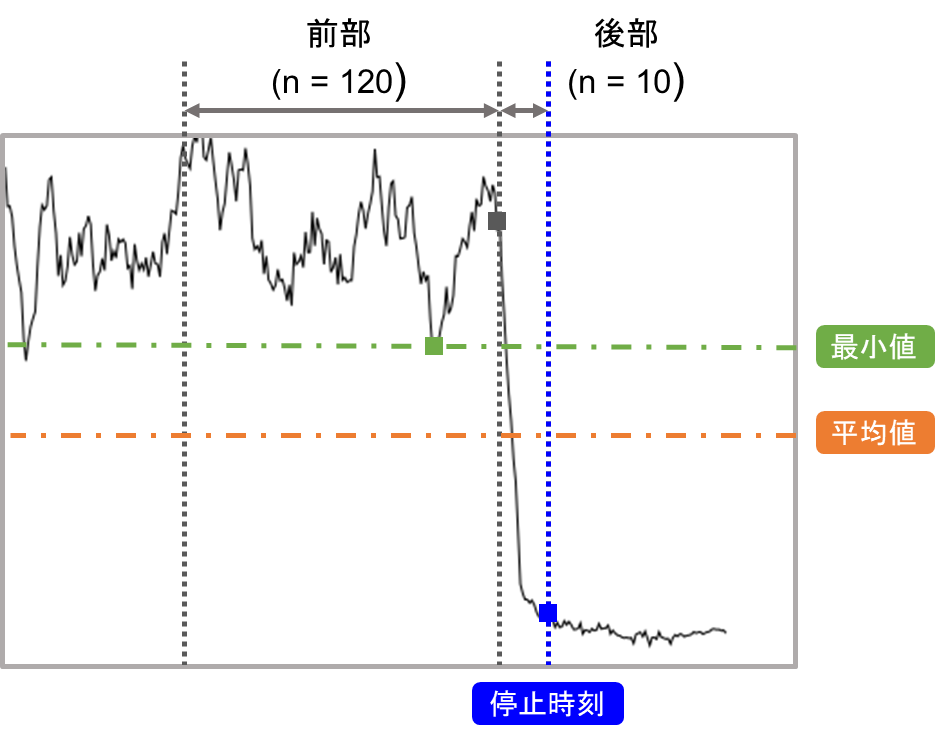
\includegraphics[width=80mm]{images/finish.png}
        \caption{Method fo detecting finish time}
    \end{center}
\end{figure}
\subsection{出力結果}
以下のように,おおよそ起動及び停止時刻を特定することができ,
他のモデルにおけるデータについても同様の結果が得られた.
\begin{figure}[htbp]
    \footnotesize
    \begin{center}
        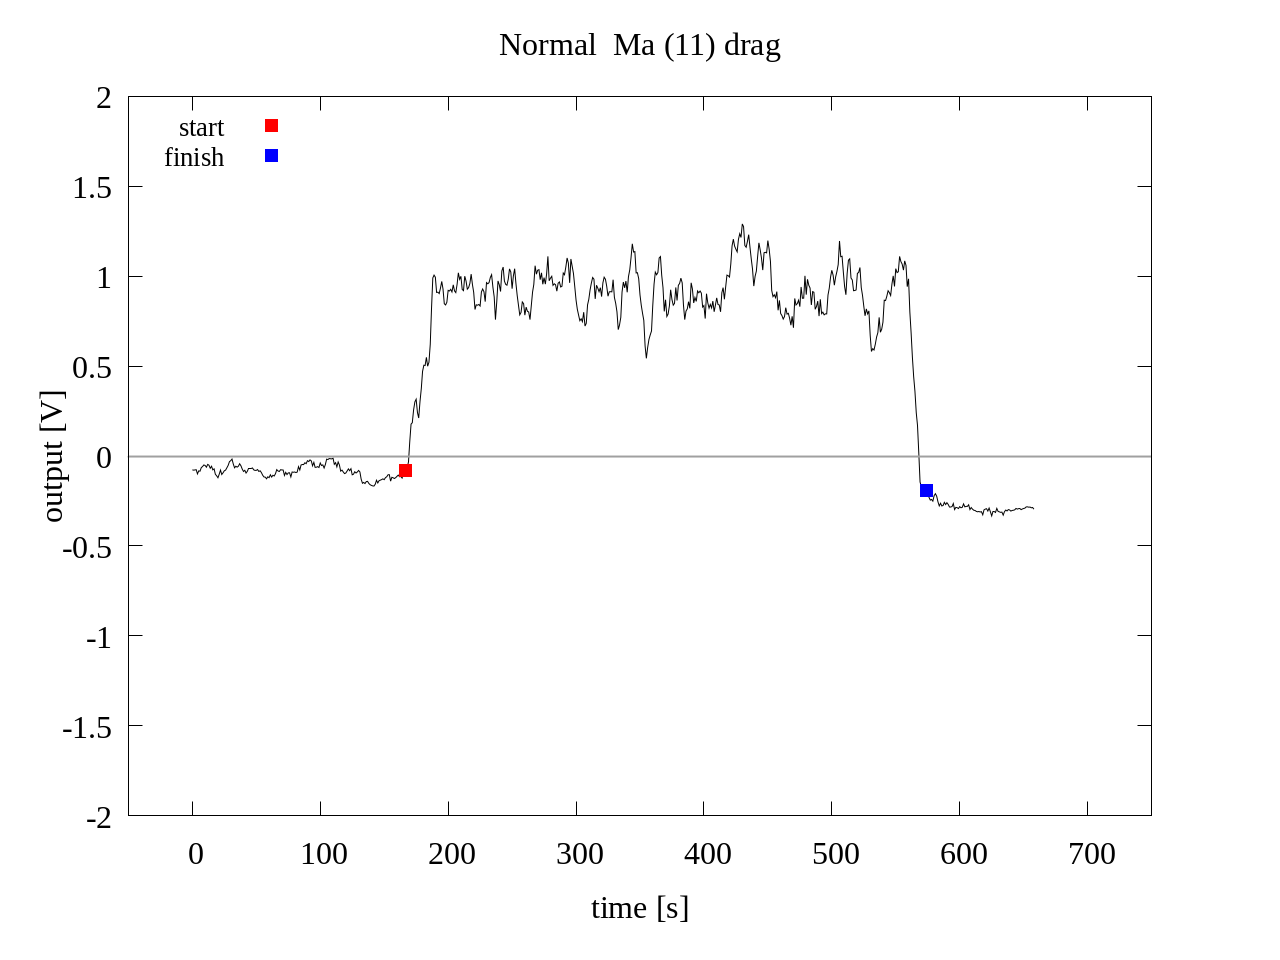
\includegraphics[width=80mm]{images/Normal_ma(11)_drag_02.png}
        \caption{Detecting start / stop time (Drag)}
        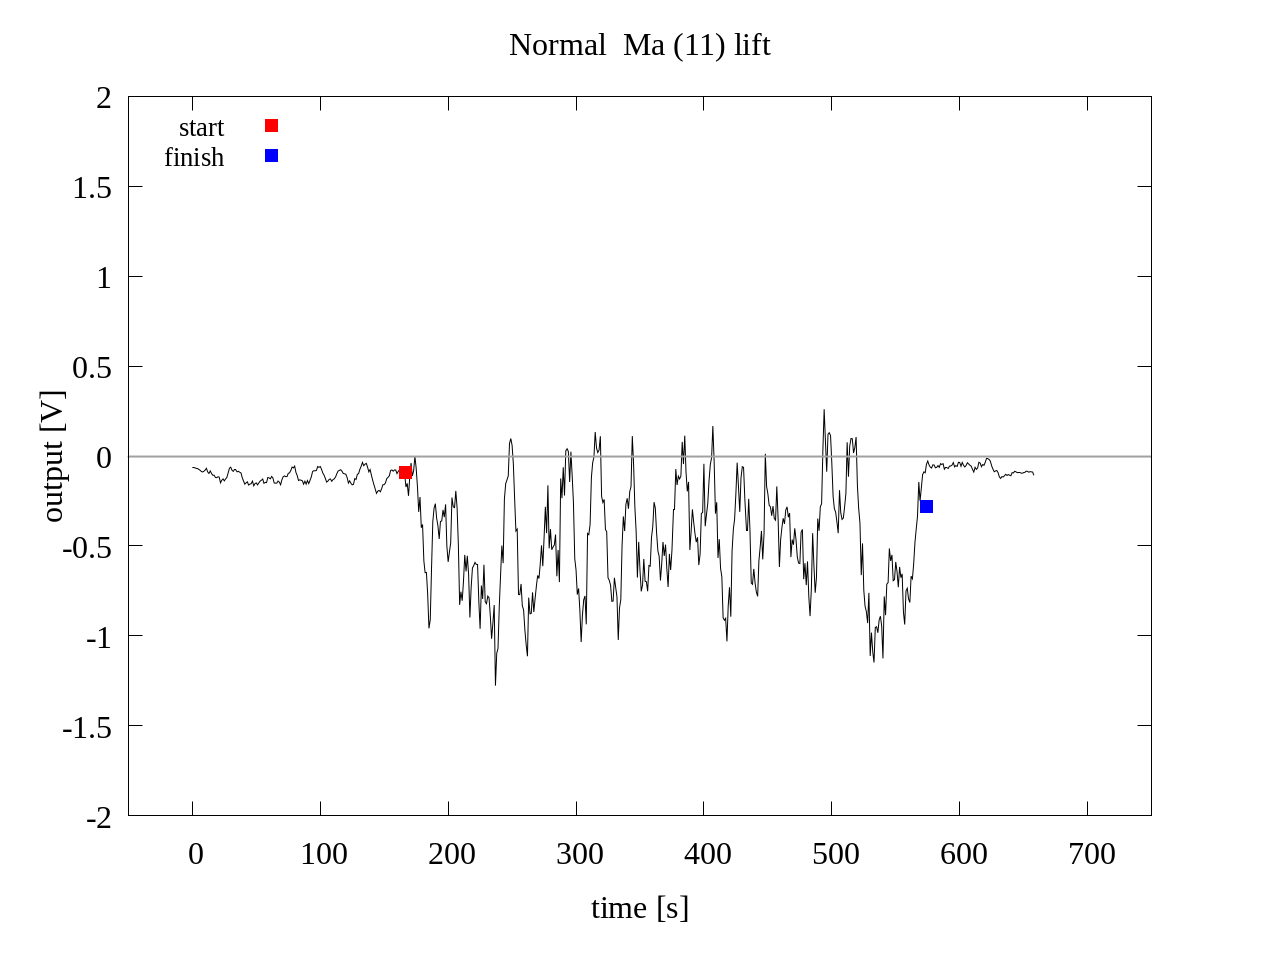
\includegraphics[width=80mm]{images/Normal_ma(11)_lift_02.png}
        \caption{Detecting start / stop time (Lift)}
    \end{center}
\end{figure}
\newpage
\section{ドリフトの補正について}
実験に使用したひずみゲージの出力結果をみると,
時刻が進むに連れて右肩下がりにドリフトするような傾向がみられた.
そのため,回流水槽の起動前,停止後のデータを用いて線形補間を行い
データに適用することとした.

\subsection{ドリフト補正のアルゴリズム}
\begin{enumerate}[(1)]
    \item 特定した起動時刻の直前(n=120)及び,停止時刻直後(n=60)の平均値を算出する.
    \item それぞれの平均値を起動時刻の60秒前,停止時刻の30秒後に適用し,それらを結んで直線を作成する.
    \item 元データから直線の差をとり,補正値として採用する.
\end{enumerate}
\subsection{出力結果}
\begin{figure}[htbp]
    \footnotesize
    \begin{center}
        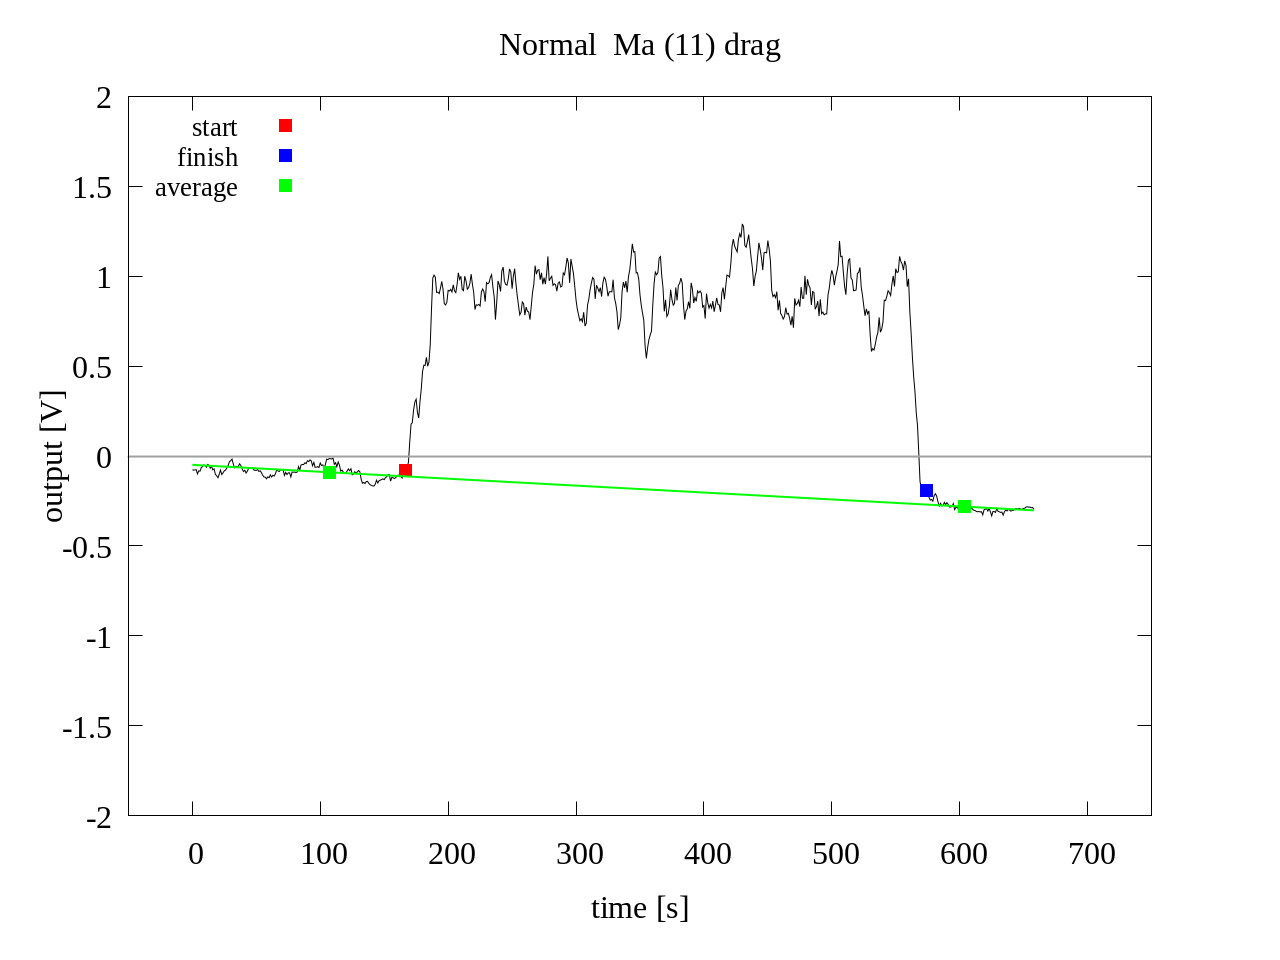
\includegraphics[width=80mm]{images/Normal_ma(11)_drag_03.png}
        \caption{Linear interpolation of start / stop time (Drag)}
    \end{center}
\end{figure}
\begin{figure}[htbp]
    \footnotesize
    \begin{center}
        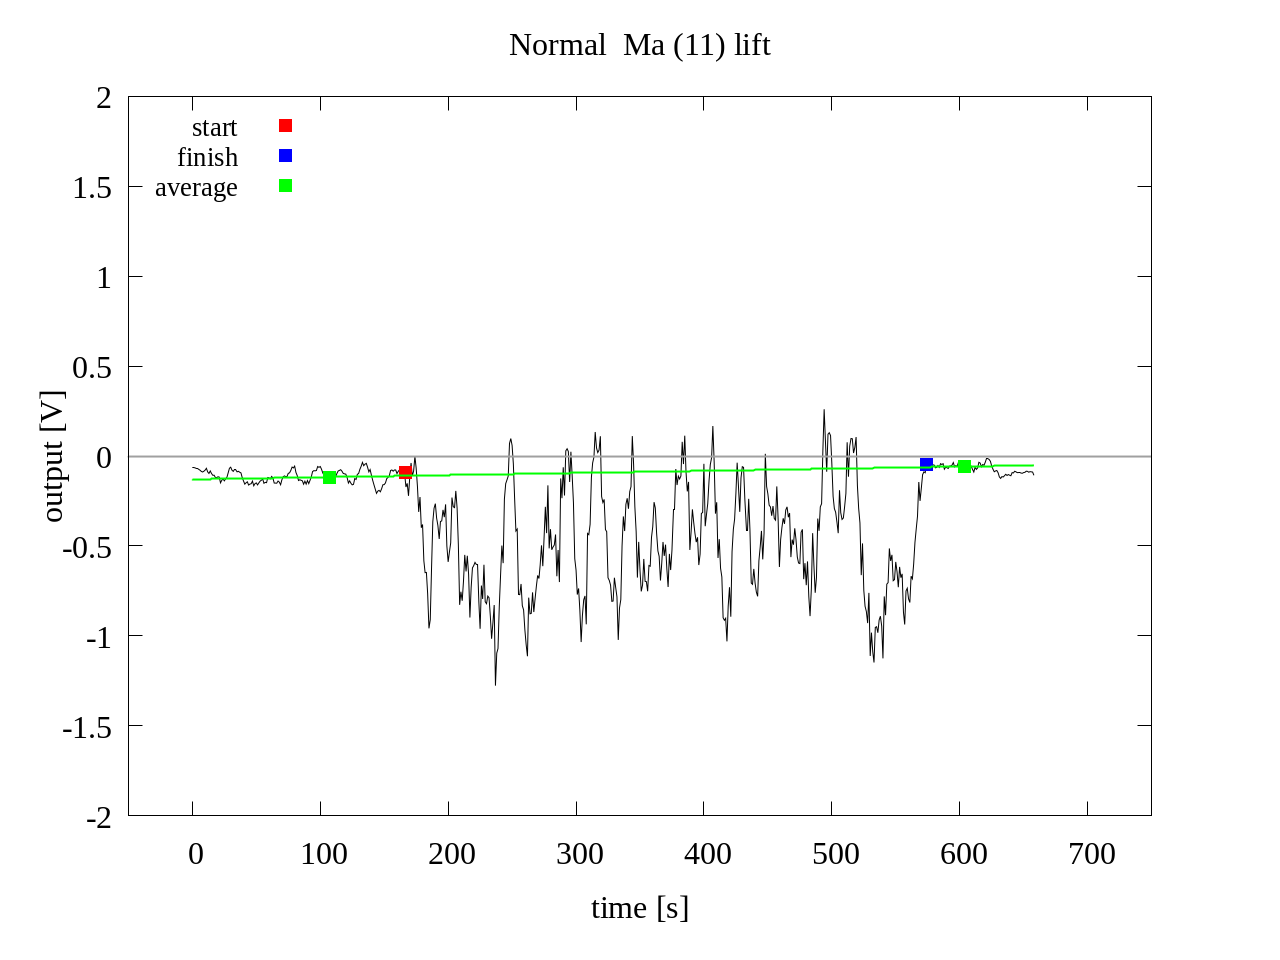
\includegraphics[width=80mm]{images/Normal_ma(11)_lift_03.png}
        \caption{Linear interpolation of start / stop time (Lift)}
    \end{center}
\end{figure}
\newpage
\section{補正結果と傾向}
\subsection{補正結果}
補正後の結果は,以下の図のようになった.
補正後のデータ(黄線)は,Drag,Liftのどちらも基準線(y=0)に沿うように移動している.
\begin{figure}[htbp]
    \footnotesize
    \begin{center}
        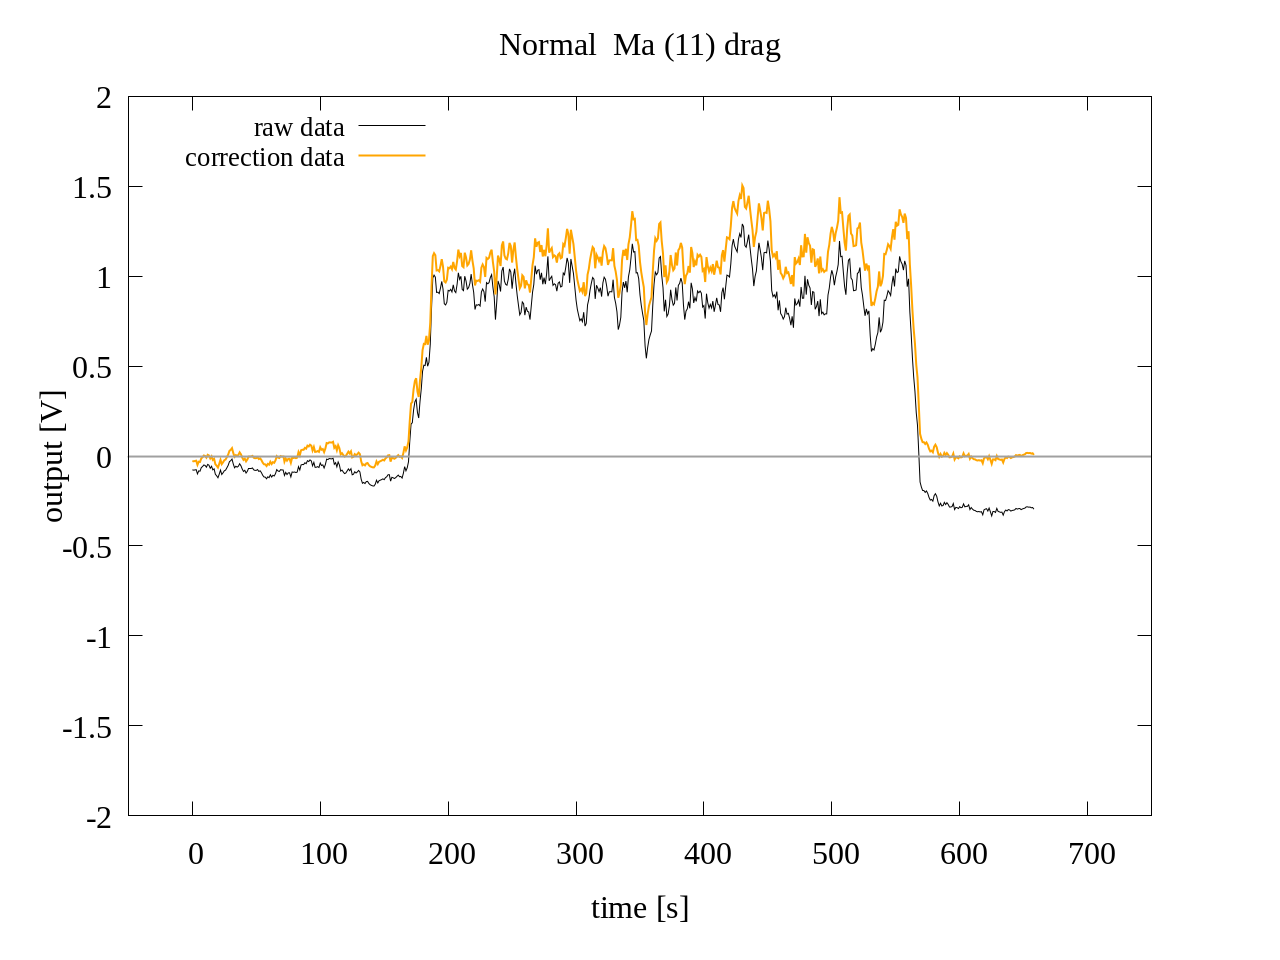
\includegraphics[width=80mm]{images/Normal_ma(11)_drag_04.png}
        \caption{Linear interpolation of start / stop time (Drag)}
        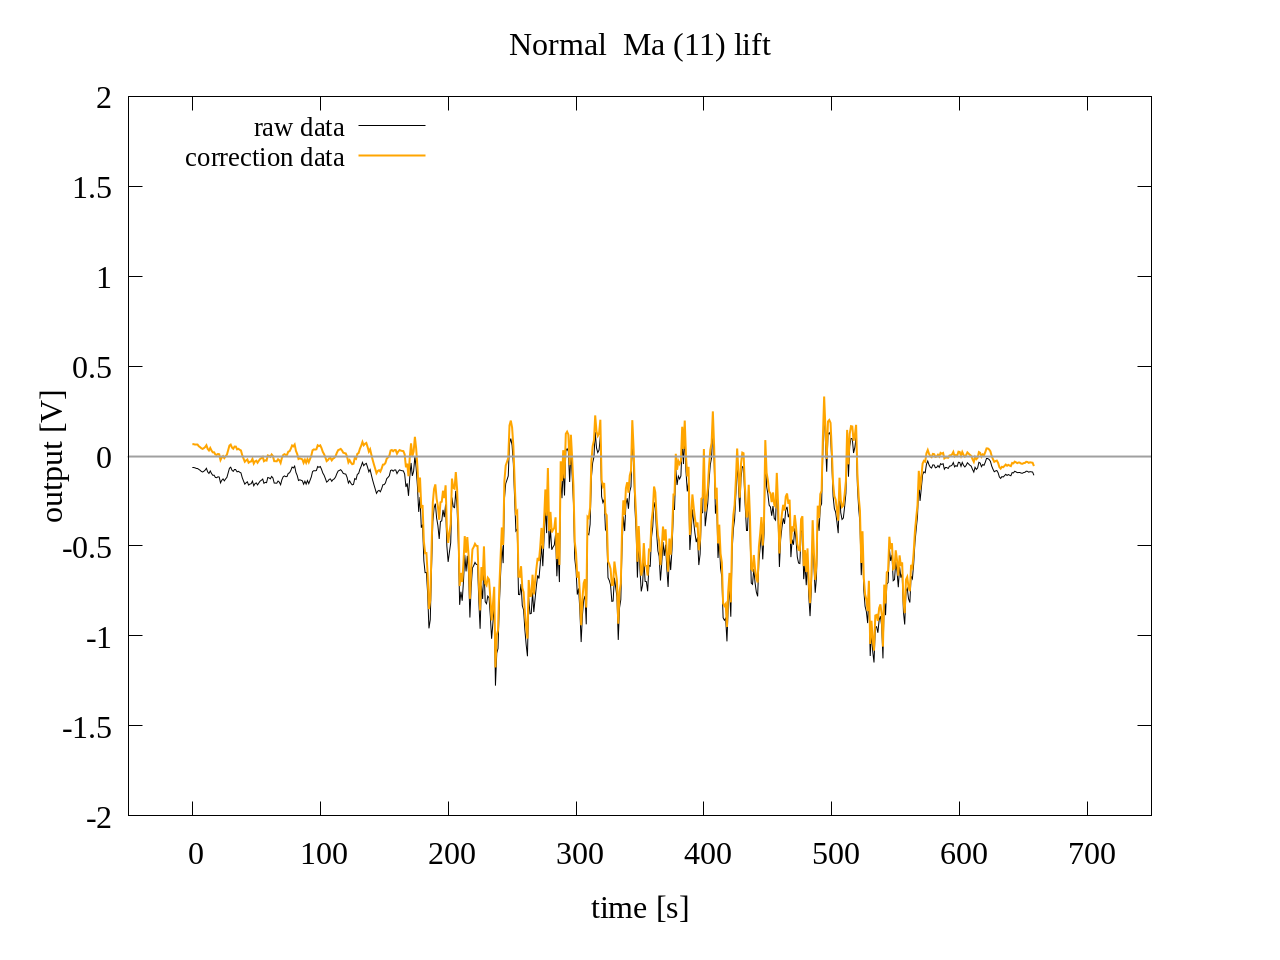
\includegraphics[width=80mm]{images/Normal_ma(11)_lift_04.png}
        \caption{Linear interpolation of start / stop time (Lift)}
    \end{center}
\end{figure}
\newpage
\subsection{平均値の比較}
補正後の出力結果から,以下の2部分に分けて平均値を算出した.
\begin{itemize}
    \item 水流の安定している範囲の出力
    \item 起動前・停止後の出力
\end{itemize}
\subsection{平均値算出のアルゴリズム}
\subsubsection{avergae (1) : 水流の安定している範囲の出力}
\begin{itemize}
    \item 特定した起動時刻の直後(n=30)及び,停止時刻直前(n=30)を除いた部分の平均値を算出する.
\end{itemize}
\subsubsection{avergae (2) : 起動前・停止後の出力}
\begin{itemize}
    \item 特定した起動時刻の直前(n=120)及び,停止時刻直後(n=60)から平均値を算出する.
\end{itemize}
\begin{figure}[htbp]
    \footnotesize
    \begin{center}
        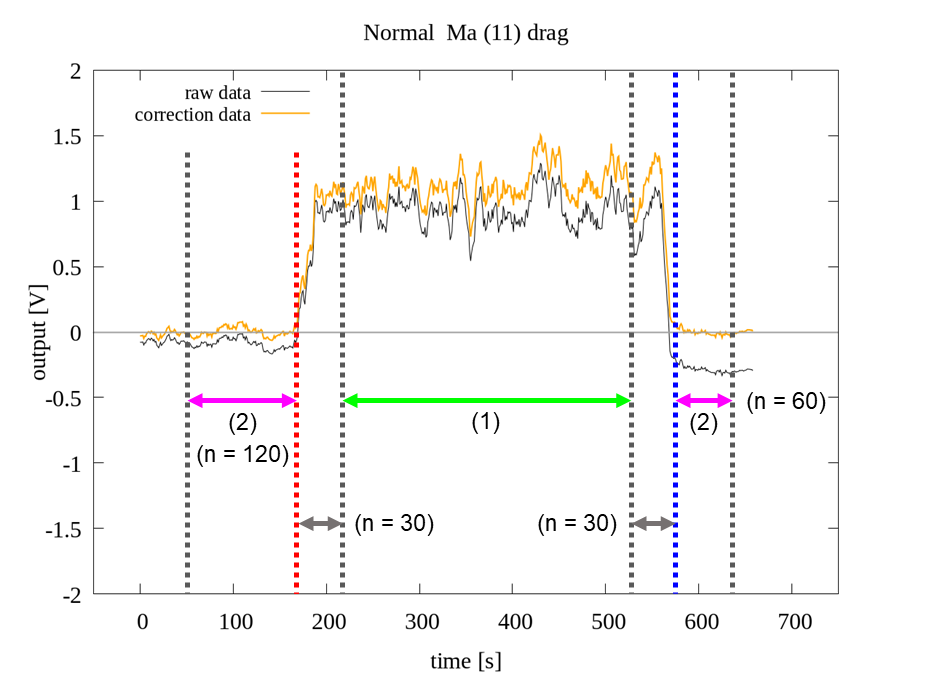
\includegraphics[width=80mm]{images/average.png}
    \end{center}
\end{figure}
\newpage
\subsection{結果}
算出した結果をプロットすると以下のようになった.\par
\begin{figure}[htbp]
    \footnotesize
    \begin{center}
        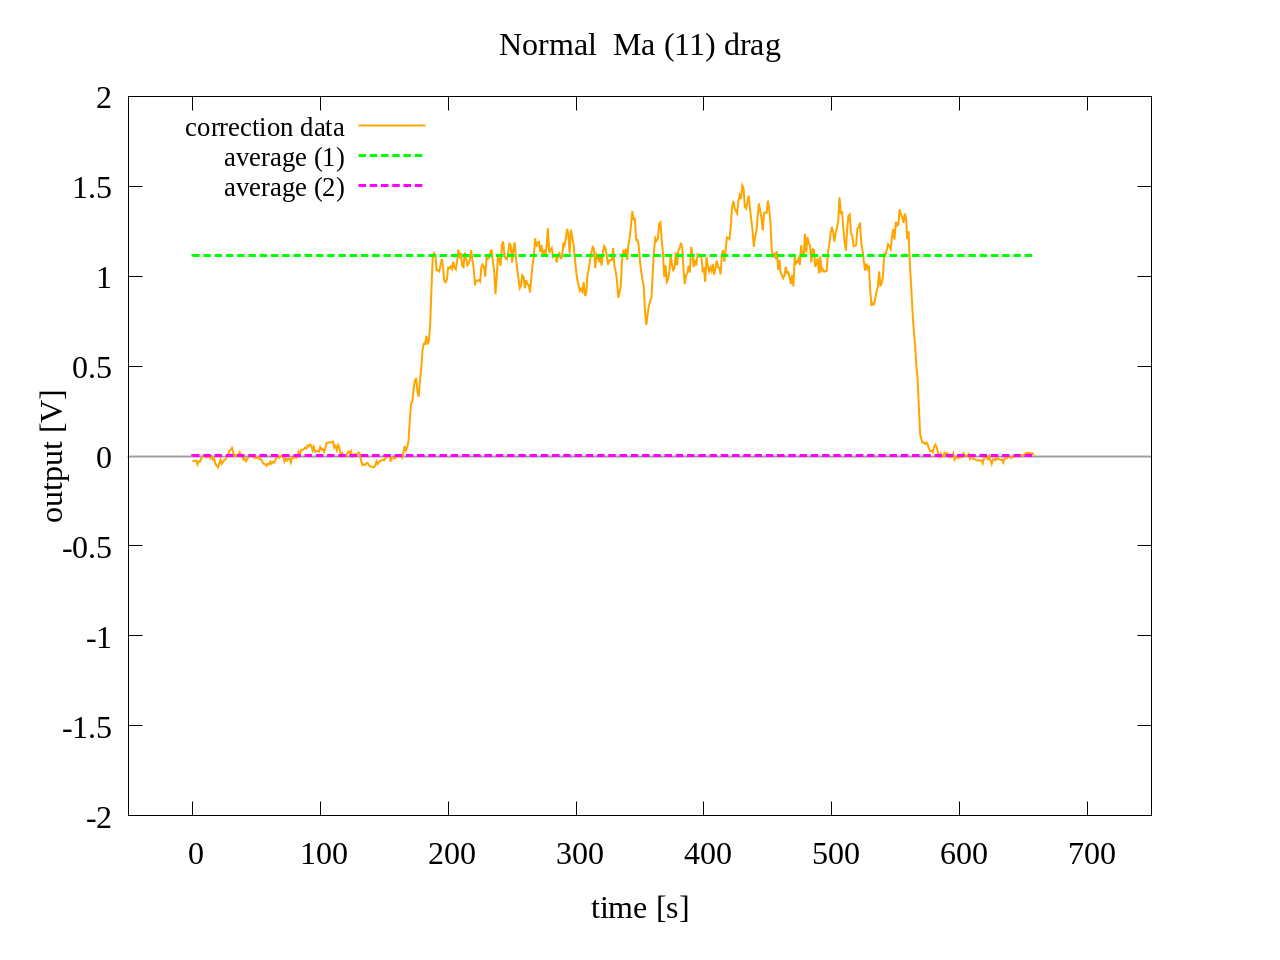
\includegraphics[width=80mm]{images/Normal_ma(11)_drag_05.png}
        \caption{Calculation of average value (Drag)}
        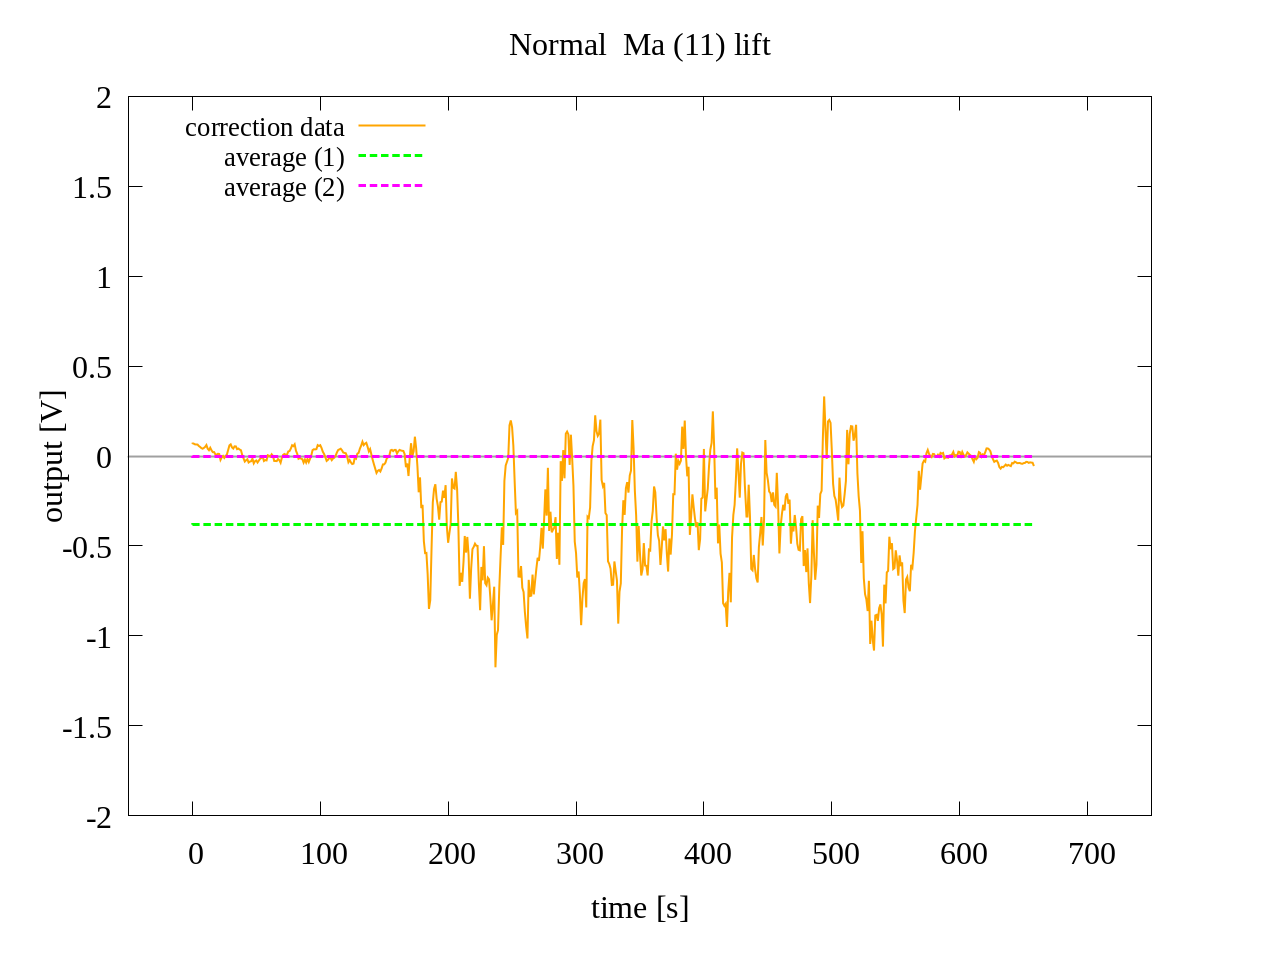
\includegraphics[width=80mm]{images/Normal_ma(11)_lift_05.png}
        \caption{Calculation of average value (Lift)}
    \end{center}
\end{figure}
また,それぞれのモデルのDragについて,算出したものを以下の表に,
2回分の実験におけるaverage(2)について表にまとめた.\par
表1をみると,average (2) は,すべての補正データにおいて
おおよそゼロに近い値を示しており,ほかの実験データについても同様な傾向が見られた.
したがって,ドリフトの補正は機能していると考えられる.\par
次に表2をみると,傾向の一致しない場合が数多くみられた.
\begin{enumerate}[※]
    \item Data(1)は2021年8月6日実施分,Data(2)は2021年7月31日実施分のデータを用いていることを示す.
\end{enumerate}
\begin{table}[htbp]
    \footnotesize
    \caption{Average of Data (1)}
    \begin{center}
        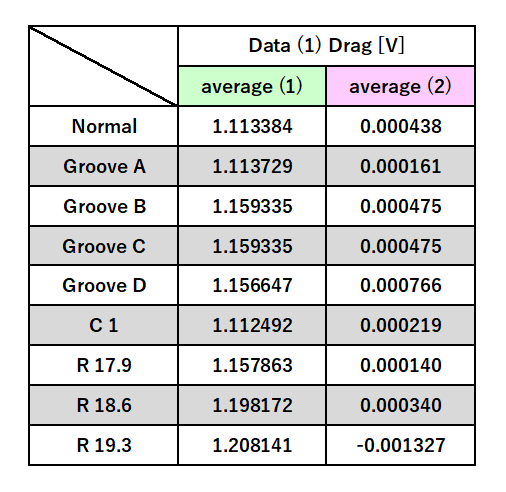
\includegraphics[width=80mm]{images/Picture2.png}
    \end{center}
\end{table}
\begin{table}[htbp]
    \footnotesize
    \caption{Average of all data}
    \begin{center}
        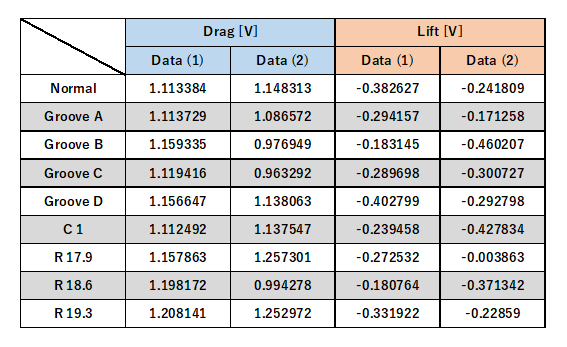
\includegraphics[width=85mm]{images/Picture1.png}
    \end{center}
\end{table}
\newpage
\subsection{考察}
今回の処理から,ドリフト補正はうまくいったが,
出力データそのものの処理が不十分であるとわかった.\par
今後は,以下のような観点からデータの解析を進めていく予定である.
\begin{itemize}
    \item ノイズ処理手法の見直し
    \item 移動平均に用いるサンプル数の見直し
    \item 補正データの再処理
\end{itemize}
\end{document}